% Turnout: 3-slide strategy deck (RISA Growth APM, Part 1). Build: ./slides/build.sh
% Every number matches the app (Bets page, engine replay of the 2025 dataset) and README.pdf.
\documentclass{article}
\usepackage[paperwidth=338.67mm,paperheight=190.5mm,margin=0mm]{geometry}
\usepackage{fontspec}
\usepackage{xcolor}
\usepackage{tikz}
\usetikzlibrary{calc}
\usepackage{tabularx}
\usepackage{array}
\usepackage{graphicx}
\usepackage{colortbl}

\setmainfont{Geist}[Path=fonts/, Extension=.ttf, UprightFont=*-Regular, BoldFont=*-SemiBold]
\setmonofont{GeistMono}[Path=fonts/, Extension=.ttf, UprightFont=*-Regular, BoldFont=*-SemiBold]
\newfontfamily\dotf{Doto-Bold.ttf}[Path=fonts/]
\newfontfamily\sym{DejaVuSans.ttf}

\definecolor{bg}{HTML}{000000}
\definecolor{fg}{HTML}{FFFFFF}
\definecolor{fg2}{HTML}{BDBDBD}
\definecolor{fg3}{HTML}{8A8A8A}
\definecolor{line}{HTML}{333333}
\definecolor{panel}{HTML}{0E0E0E}
\definecolor{dim}{HTML}{5A5A5A}
\pagecolor{bg}\color{fg}
\pagestyle{empty}
\setlength{\parindent}{0pt}
\setlength{\tabcolsep}{4.5pt}
\renewcommand{\arraystretch}{1.2}
\arrayrulecolor{line}

% --- helpers ---------------------------------------------------------------
\newcommand{\fs}[2]{\fontsize{#1}{#2}\selectfont}
\newcommand{\tg}[1]{\,{\fs{6.8}{8}\ttfamily\color{fg3}[#1]}}        % evidence tag
\newcommand{\lab}[1]{{\fs{8}{10}\ttfamily\color{fg3}\MakeUppercase{#1}}}
\newcommand{\hd}[1]{{\fs{7.6}{9}\ttfamily\color{fg3}\MakeUppercase{#1}}}
\newcommand{\gS}{{\sym ●}}  % scale   (same glyphs as the app)
\newcommand{\gW}{{\sym ◐}}  % watch / change
\newcommand{\gX}{{\sym ○}}  % stop
\newcolumntype{L}{>{\raggedright\arraybackslash}X}
\newcolumntype{P}[1]{>{\raggedright\arraybackslash}p{#1}}
\newcolumntype{R}[1]{>{\raggedleft\arraybackslash}p{#1}}

% \blk{x}{y}{width}{content}: block at (x, y) cm from the top-left corner
\newcommand{\blk}[4]{\node[anchor=north west,inner sep=0pt] at (#1,-#2) {\begin{minipage}[t]{#3cm}#4\end{minipage}};}
\newcommand{\panel}[4]{\draw[line,rounded corners=6pt,fill=panel] (#1,-#2) rectangle ++(#3,-#4);}

\newcommand{\chrome}[3]{%
  \blk{1.3}{0.72}{22}{\fs{8.4}{10}\ttfamily\color{fg3}\textcolor{bg}{\colorbox{fg}{\textbf{TURNOUT}}}\enspace RISA GROWTH APM · CHALLENGE A: ATTENDEE GROWTH · BENGALURU · SLIDE #1/3}
  \blk{22.6}{0.72}{9.97}{\raggedleft\fs{8.4}{10}\ttfamily\color{fg}\textbf{G L LOHITH}}
  \draw[line] (1.3,-1.4) -- (32.57,-1.4);
  \blk{1.3}{1.7}{31.3}{\fs{26}{29}\bfseries #2}
  \blk{1.3}{2.9}{31.3}{\fs{11}{13.6}\color{fg2}#3}
  \draw[line] (1.3,-18.0) -- (32.57,-18.0);
}
\newcommand{\footer}[1]{\blk{1.3}{18.18}{31.3}{\fs{7.6}{9.2}\color{fg3}#1}}

\begin{document}
% ===========================================================================
% SLIDE 1: HOW HIGH CAN WE AIM?
% ===========================================================================
\begin{tikzpicture}[remember picture,overlay,every node/.append style={text=fg}]
\begin{scope}[shift={(current page.north west)}]
\chrome{1}{How high can we aim? \textcolor{fg3}{Demand for 2,988 visitors, +46\% on 2025}}{\textbf{G L Lohith} · Challenge A: Attendee Growth, CampusFest (12–13 Apr) · \textbf{City: Bengaluru}, because Bengaluru Urban has \textbf{1,148 colleges, the most of any district in India}\tg{S1} (Pune 517, Hyderabad 465): the densest ground for the peer channels we bet on.}

% ---- four headline numbers ------------------------------------------------
\foreach \x in {1.3, 9.22, 17.14} \panel{\x}{3.95}{7.5}{3.55}
\draw[fg,rounded corners=6pt,line width=0.9pt] (25.06,-3.95) rectangle ++(7.51,-3.55);
\blk{1.7}{4.22}{6.8}{\lab{Base · today's rates}\\[1pt]{\dotf\fs{44}{46}2,097}\\[4pt]
  {\fs{8.6}{10.8}\color{fg2}+2\% on 2025 (2,050)\tg{D} · ₹143 per visitor\\3,108 registrations, no new levers}}
\blk{9.62}{4.22}{6.8}{\lab{Goal · organisers' target}\\[1pt]{\dotf\fs{44}{46}2,200}\\[4pt]
  {\fs{8.6}{10.8}\color{fg2}raised from 1,800 to 2,200 on 15 Mar\tg{D}\\needs 3,262 registrations at base rates\tg{calc}}}
\blk{17.54}{4.22}{6.8}{\lab{Plan · funded on slide 2}\\[1pt]{\dotf\fs{44}{46}2,282}\\[4pt]
  {\fs{8.6}{10.8}\color{fg2}\textbf{104\% of goal}, +11\% on 2025 · ₹120 per visitor\\→ 2,418 when the reserve follows winners}}
\blk{25.46}{4.22}{6.8}{\lab{Stretch · demand ceiling}\\[1pt]{\dotf\fs{44}{46}2,988}\\[4pt]
  {\fs{8.6}{10.8}\color{fg2}\textbf{+46\% on 2025} · ₹100 per visitor\\4,196 registrations; needs the capacity lever}}

% ---- column A: who we target ---------------------------------------------
\blk{1.3}{7.95}{10.1}{\fs{12}{14}\bfseries Who we target first, and why
  \\[5pt]\fs{8.5}{10.2}
  \begin{tabularx}{10.1cm}{@{}P{2.75cm}R{1.3cm}R{1.75cm}R{0.9cm}L@{}}
  \hd{Segment} & \hd{Students} & \hd{Reach·ID·Reg} & \hd{Reg.} & \hd{Why first} \\\hline
  1 Clubs \& societies & 60,000 & 10·9·85\% & 459 & one lead signs up 10–30 \\
  2 Engineering \& tech & 2,40,000 & 5·12·80\% & 1,152 & densest; 37\% of plan \\
  3 Friends of registrants & 20,000 & 25·8·80\% & 320 & pre-qualified, ~free \\
  4 Management \& design & 90,000 & 6·10·78\% & 421 & small, high intent \\
  5 Arts, sci., commerce & 4,20,000 & 3·8·75\% & 756 & largest but cold \\\hline
  \textbf{Total} & \textbf{8,30,000} & \textbf{41,000 reached} & \textbf{3,108} & \\
  \end{tabularx}
  \\[5pt]{\fs{8}{10}\color{fg2}Students: ≈8–10 lakh, derived from AISHE\tg{A·S1}; segment rates are planning assumptions\tg{A}.
  \textbf{Overlap:} friends (20,000) also sit in segments 1–5, an overcount of ≤2.4\%; the app dedupes people by ID.\\[3pt]
  \textbf{Not first:} alumni and the general public. There's no campus channel to reach them and intent is lowest; walk-ins (5\%) cover the public\tg{A}.}}

% ---- column B: funnel maths ----------------------------------------------
\blk{11.8}{7.95}{10.1}{\fs{12}{14}\bfseries The funnel, stage by stage}
\foreach \x/\t in {11.8/STAGE, 14.0/{DOTS (LOG)}, 17.1/{BASE · CONV.}, 19.75/{STRETCH}} \node[anchor=west,inner sep=0] at (\x,-8.75) {\fs{7.4}{8}\ttfamily\color{fg3}\t};
\foreach \name/\dots/\base/\str/\y in {%
  Students/30/{8,30,000}/{8,30,000}/9.3,
  Reached/18/{41,000 · 4.9\%}/{51,250 ×1.25}/9.95,
  Identified/8/{3,928 · 9.6\%}/{4,910 · 9.6\%}/10.6,
  Registered/7/{3,108 · 79.1\%}/{4,196 · 85.5\%}/11.25,
  Confirmed/6/{2,766 · 89\%}/{3,735 · 89\%}/11.9,
  Attended/4/{1,992 · 72\%}/{2,838 · 76\%}/12.55,
  + walk-ins/1/{105 · 5\%}/{149 · 5\%}/13.2}{
  \node[anchor=west,inner sep=0] at (11.8,-\y) {\fs{9}{10}\name};
  \foreach \i in {1,...,\dots} \fill[fg] (13.9+\i*0.1,-\y) circle (0.045);
  \node[anchor=west,inner sep=0] at (17.1,-\y) {\fs{8.1}{10}\ttfamily\base};
  \node[anchor=west,inner sep=0] at (19.75,-\y) {\fs{8.1}{10}\ttfamily\color{fg2}\str};
}
\draw[line] (11.8,-13.6) -- (21.9,-13.6);
\node[anchor=west,inner sep=0] at (11.8,-14.0) {\fs{10}{11}\bfseries Visitors};
\foreach \i in {1,...,5} \fill[fg] (13.9+\i*0.1,-14.0) circle (0.045);
\node[anchor=west,inner sep=0] at (17.1,-14.0) {\fs{9.5}{11}\ttfamily\bfseries 2,097};
\node[anchor=west,inner sep=0] at (19.75,-14.0) {\fs{9.5}{11}\ttfamily\bfseries 2,988};
\blk{11.8}{14.4}{10.1}{\fs{8}{10}\color{fg2}
  {\ttfamily visitors = registered × confirm × show-up ÷ (1 − walk-in share)\\
  base\ \ \ \ 3,108 × 0.89 × 0.72 ÷ 0.95 = 2,097\\
  stretch 4,196 × 0.89 × 0.76 ÷ 0.95 = 2,988}\\[4pt]
  \textbf{Identified → registered:} our plan uses \textbf{79.1\%}, in line with 2025's full campaign, \textbf{80.0\%} (to 20 Apr)\tg{D}. The organisers' targets imply 88.9\% (3,200 ÷ 3,600); on 31 Mar the data stood at 70.4\%\tg{D}, the gap slide 2 attacks.}

% ---- column C: stretch levers + risk -------------------------------------
\blk{22.3}{7.95}{10.27}{\fs{12}{14}\bfseries What makes stretch higher than base
  \\[5pt]\fs{8.5}{10.2}
  \begin{tabularx}{10.27cm}{@{}P{1.75cm}P{2.1cm}LR{0.85cm}@{}}
  \hd{Lever} & \hd{Base→stretch} & \hd{How we pull it} & \hd{Adds} \\\hline
  Reach & 41,000 → 51,250 & +10 ambassador colleges, +20 clubs (bets 1–2) & +524 \\
  Registration & 79.1 → 85.5\% & one-tap RSVP; group form for club leads & +210 \\
  Show-up & 72 → 76\%\tg{S2} & reminders at 48 h and on the morning; groups arrive together & +157 \\
  Capacity & 2,500 total → per day\tg{A} & day-2 passes, staggered entry slots & frees 488 \\\hline
  & & \textbf{2,097 → 2,988} & \\
  \end{tabularx}
  \\[3pt]{\fs{8}{10}\color{fg2}2025's day 1 took 70\% of visitors\tg{D}, so 2,988 means ≈2,090 on day 1: under 2,500 per day. Without the lever, the app's total cap holds stretch to 2,500.}}
\draw[fg,dashed,rounded corners=6pt,line width=0.6pt] (22.3,-14.25) rectangle ++(10.27,-3.45);
\blk{22.65}{14.5}{9.6}{\lab{Riskiest assumption: show-up 72\%}\\[3pt]
  {\fs{9}{11.3}Unknowable until the gates open\tg{S2}. \textbf{At 60\%, base falls from 2,097 to 1,747} (−350); each point is ≈29 visitors.}\\[3pt]
  {\fs{8}{10}\color{fg2}Hedge: plan registrations 10\% over need (≈3,590), track the confirm rate weekly as its early proxy, send reminders.}}

\footer{\textbf{Evidence:} [S] sourced · [D] 2025 RISA attendee dataset, replayed in the app · [A] our assumption · [calc] derived.\quad S1 AISHE 2023-24 · S2 PheedLoop Event Data Lab 5: free-event no-show ≈28\%, large free events ≈24\%.\quad \textbf{Full calculations and sensitivity: README.pdf §4–§5.}}
\end{scope}
\end{tikzpicture}
\newpage

% ===========================================================================
% SLIDE 2: WHERE WILL WE PLACE OUR BETS?
% ===========================================================================
\begin{tikzpicture}[remember picture,overlay,every node/.append style={text=fg}]
\begin{scope}[shift={(current page.north west)}]
\chrome{2}{Where will we place our bets? \textcolor{fg3}{Money follows evidence}}{Five bets ranked by \textbf{RICE = Reach × Impact × Confidence ÷ Effort}. The two strongest get \textbf{65\% of committed spend}. The two weakest get capped tests and earn more only by crossing their scale line; a \textbf{₹25,000 reserve} goes to whichever bets do.}

\blk{1.3}{3.95}{31.27}{\fs{8.5}{10.2}
\begin{tabularx}{31.27cm}{@{}P{0.4cm}P{6.4cm}P{2.6cm}P{2.3cm}P{2.3cm}P{3.6cm}LP{3.7cm}@{}}
\hd{\#} & \hd{Idea · why it works} & \hd{RICE (R·I·C÷E)} & \hd{Lift · of goal} & \hd{Budget · ₹/vis.} & \hd{People · timeline} & \hd{How we test it (first 14 days)} & \hd{KPI to watch} \\\hline
\textbf{1} & \textbf{Campus ambassadors.} Peers in the top 40 colleges turn interest into registrations; trust lifts show-up. & 40k·2·0.8÷6 \newline \textbf{10,667} & \textbf{659} · 30\% & ₹1,00,000 \newline {\color{fg3}₹152} & Meera Iyer + 40 ambassadors · 6 pw · 25 Jan–11 Apr & 10 colleges live, 10 held out; compare registrations per identified student. & CPR ≤ ₹50; ≥ 8 regs/day \\
\textbf{2} & \textbf{Club group sign-ups.} One club lead brings 10–30 members, who confirm and arrive together. & 25k·2·0.8÷4 \newline \textbf{10,000} & \textbf{689} · 31\% & ₹80,000 \newline {\color{fg3}₹116} & Meera Iyer + a club lead · 4 pw · 28 Jan–11 Apr & 15 clubs on a group form vs individual links; compare group size and confirm rate. & CPR ≤ ₹50; confirm ≥ 88\% \\
\textbf{3} & \textbf{Bring-3-friends referrals.} Friends of registrants are pre-qualified; the only cost is the reward. & 15k·2·0.7÷3 \newline \textbf{7,000} & \textbf{355} · 16\% & ₹30,000 \newline {\color{fg3}₹85} & Dev Malhotra · 3 pw · 12 Feb–11 Apr & A/B the reward (merch vs priority entry); dedupe referred IDs. & CPR ≤ ₹45; ≥ 6/day; confirm ≥ 88\% \\
\textbf{4} & \textbf{Creator reels} (test). Student creators reach the large, cold arts and commerce segment. & 80k·1·0.4÷5 \newline \textbf{6,400} & \textbf{59} · 3\% & ₹20,000 test \newline {\color{fg3}₹337} & Nisha Rao · 5 pw · 10 Feb–11 Apr & 3 creators × 2 weeks on tracked links; more money only past the scale line. & CPR ≤ ₹70; confirm ≥ 88\% \\
\textbf{5} & \textbf{Paid retargeting} (test). Re-reaches landing-page visitors who didn't finish. & 120k·0.5·0.4÷4 \newline \textbf{6,000} & \textbf{55} · 2\% & ₹15,000 test \newline {\color{fg3}₹274} & Arjun Verma · 4 pw · 1 Feb–11 Apr & Retargeting audiences only, fresh creatives, hard cap. & CPR ≤ ₹80; confirm ≥ 88\% \\\hline
& \textbf{Bets total} & & \textbf{1,817} · 83\% & \textbf{₹2,45,000} & \multicolumn{3}{l}{\color{fg2}₹3,00,000 = bets ₹2,45,000 + always-on ₹30,000 + reserve ₹25,000} \\
\end{tabularx}}

% ---- incremental waterfall ------------------------------------------------
\blk{1.3}{11.2}{31.27}{\fs{10}{12}\bfseries Each bet's lift over a no-bet baseline\fs{8.3}{10}\mdseries\color{fg2}\enspace· lift = budget ÷ the channel's 2025 cost per verified visitor; spend above the 2025 level at 2× that cost\tg{D·A}}
\def\u{0.0101}% cm per visitor: 3,000 = 30.3 cm
\foreach \lbl/\v/\x/\c/\t in {{baseline 465}/465/0/dim/fg, {B1 +659}/659/465/fg/bg, {B2 +689}/689/1124/fg2/bg, {B3 +355}/355/1813/fg/bg, {}/59/2168/fg2/bg, {}/55/2227/fg/bg}{
  \fill[\c] (1.3+\x*\u+0.03,-12.15) rectangle (1.3+\x*\u+\v*\u-0.03,-12.85);
  \node[anchor=west,inner sep=0] at (1.3+\x*\u+0.12,-12.5) {\fs{8.3}{9}\ttfamily\textcolor{\t}{\lbl}};
}
\draw[fg,dashed,line width=0.6pt] (1.3+2282*\u+0.03,-12.15) rectangle (1.3+2418*\u-0.03,-12.85);
\foreach \v/\t/\a in {2050/{2025: 2,050}/south east, 2200/{goal 2,200}/south west, 2988/{stretch 2,988}/south east}{
  \draw[fg2,line width=0.7pt] (1.3+\v*\u,-11.95) -- (1.3+\v*\u,-13.05);
  \node[anchor=\a,inner sep=1pt] at (1.3+\v*\u,-11.95) {\fs{7.8}{8}\ttfamily\color{fg2}\t};
}
\node[anchor=north,inner sep=1pt] at (1.3+2282*\u,-13.05) {\fs{7.8}{8}\ttfamily\bfseries plan 2,282};
\node[anchor=north west,inner sep=1pt] at (1.3+2418*\u+0.1,-13.05) {\fs{7.8}{8}\ttfamily\color{fg2}+ reserve → 2,418};
\blk{1.3}{13.55}{31.27}{\fs{8.2}{10}\color{fg2}\textbf{No-bet baseline 465} = always-on organic search and community groups at their 2025 spend (₹30,000 → 360)\tg{D} + walk-ins 105\tg{A}. B4 and B5 add 59 and 55. The 2,097 base case on slide 1 already assumes these channels run at today's rates; this chart shows what each bet adds. Each person counts once, by registration source.}

% ---- bottom three columns -------------------------------------------------
\panel{1.3}{14.6}{10.1}{3.2}
\blk{1.65}{14.85}{9.4}{\lab{Double down: bets 1 and 2}\\[2pt]\fs{8.6}{10.6}
  The top two RICE scores, aimed at the weakest stage: identified→registered was 70.4\% on 31 Mar against the 88.9\% the organisers' targets imply\tg{D}. Both were under the scale line that day (₹35, ₹49 vs ₹58.86)\tg{D}. \textbf{₹1,80,000}, plus first call on the reserve.}
\panel{11.8}{14.6}{10.1}{3.2}
\blk{12.15}{14.85}{9.4}{\lab{Deprioritise or reject}\\[2pt]\fs{8.6}{10.6}
  \textbf{5 Retargeting} drops from the largest line to a \textbf{₹15,000 test}: in 2025 it reached ₹256 per registration\tg{D}. \textbf{4 Reels}: a ₹20,000 test first.
  \textbf{Rejected:} a paid headliner (far over budget) and city-wide outdoor ads (no attribution, so no way to test).}
\panel{22.3}{14.6}{10.27}{3.2}
\blk{22.65}{14.85}{9.6}{\lab{Constraints}\\[2pt]\fs{8.4}{10.3}
  \textbf{Dependencies:} referrals need registrants from bets 1–2; retargeting needs their traffic. \textbf{Overlaps:} people deduped by ID, one source each. \textbf{Risks:} ambassador fatigue; a few big clubs carry bet 2; Meera owns both top bets (add a co-owner); reward abuse.}

\footer{RICE: reach = students in the period · impact 0.25–3 · confidence 0–1 · effort = person-weeks (Intercom). Lifts and budgets are planning figures\tg{A} built on 2025 costs per visitor\tg{D}; they are live on the app's Bets page.\quad \textbf{Scoring and lifts: README.pdf §6.}}
\end{scope}
\end{tikzpicture}
\newpage

% ===========================================================================
% SLIDE 3: HOW WILL WE KNOW WHAT'S WORKING?
% ===========================================================================
\begin{tikzpicture}[remember picture,overlay,every node/.append style={text=fg}]
\begin{scope}[shift={(current page.north west)}]
\chrome{3}{How will we know what's working?}{Each bet has leading indicators with \textbf{scale / change / stop} lines, judged by the app at fixed checkpoints. Money moves only on evidence. The last column is the app's reading at the \textbf{31 Mar decision point}, replaying the 2025 data.}

\blk{1.3}{3.95}{31.27}{\fs{8.5}{10.2}
\begin{tabularx}{31.27cm}{@{}P{2.35cm}P{4.2cm}P{3.0cm}P{4.6cm}P{4.0cm}LP{3.9cm}@{}}
\hd{Bet} & \hd{Variable · biggest risk} & \hd{Early signal (window)} & \hd{\gS{} Scale line → action} & \hd{\gW{} Change zone → action} & \hd{\gX{} Stop · 2nd reading in a row → action} & \hd{31 Mar reading (app)} \\\hline
\textbf{1 Ambassadors} & regs per active ambassador · fatigue & CPR 14 d; regs/day 7 d & ≤ ₹50 and ≥ 8/day → reserve tranche, +10 colleges & ₹50–120 → swap weak ambassadors & ≥ ₹120 or ≤ 3/day → pause; money to bet 2 & \gS{} \textbf{Scale}: ₹35, 8.7/day \\
\textbf{2 Club sign-ups} & members per lead · a few big clubs & CPR 14 d; confirm 6 wk & ≤ ₹50 and confirm ≥ 88\% → tranche, +20 clubs & confirm 78–88\% → reminders via club leads & ≥ ₹120 or confirm ≤ 78\% → no new clubs & \gW{} \textbf{Watch}: ₹49 ok, confirm 85.4\% \\
\textbf{3 Referrals} & referrals per registrant · reward abuse & CPR; regs/day; confirm & ≤ ₹45, ≥ 6/day and confirm ≥ 88\% → raise the reward & in between → A/B the reward & ≥ ₹110, ≤ 2/day or confirm ≤ 78\% → end it & \gW{} \textbf{Watch}: ₹30, 8.7/day ok; confirm 82.0\% \\
\textbf{4 Reels (test)} & clicks→regs per creator · views don't convert & CPR 14 d; confirm & ≤ ₹70 and confirm ≥ 88\% → release next ₹20,000 & ₹70–130 → new brief, new call to action & ≥ ₹130 or confirm ≤ 78\% → end the test & \gX{} \textbf{Stop}: ₹134, confirm 77.7\% \\
\textbf{5 Retargeting (test)} & marginal CPR · weak show-up & CPR 14 d; confirm & ≤ ₹80 and confirm ≥ 88\% → release next ₹15,000 & ₹80–150 → refresh creatives & ₹150 bet line or ₹110 portfolio line, \emph{whichever comes first} → end & \gX{} \textbf{Stop}: ₹256 on 75 registrations \\\hline
\textbf{Portfolio rule} & \multicolumn{2}{l}{\color{fg2}every campaign vs portfolio CPR (14 d, ≥ 15 regs)} & ≤ 0.8× portfolio (≤ ₹58.86) & weak CTR, form starts, cancels & ≥ 1.5× portfolio (≥ ₹110.37) & \color{fg2}2 stop, 5 scale\tg{D} \\
\end{tabularx}}

% ---- checkpoint timeline -------------------------------------------------
\blk{1.3}{11.0}{14}{\fs{11.5}{13}\bfseries Checkpoints, so we adapt before it's too late}
\draw[fg3,line width=0.7pt] (2.2,-12.45) -- (14.8,-12.45);
\foreach \x/\top/\bot in {
  2.2/{Day 0}/{launch, baseline},
  4.0/{Day 7}/{first read: CTR, regs/day},
  5.8/{Day 14}/{first verdict, ≥15 regs},
  7.6/{Weekly}/{Monday: what moved},
  9.4/{31 Mar}/{decision point, 11 days left},
  11.2/{11 Apr}/{registration closes},
  13.0/{12–13 Apr}/{show-up measured},
  14.8/{+14 days}/{decision outcomes}}{
  \fill[fg] (\x,-12.45) circle (0.11);
  \node[anchor=south,inner sep=0] at (\x,-12.2) {\fs{8}{9}\ttfamily\bfseries\top};
  \node[anchor=north,inner sep=0,text width=1.75cm,align=center] at (\x,-12.7) {\fs{7.6}{8.8}\color{fg2}\bot};
}
\blk{1.3}{14.25}{14}{\fs{8.5}{10.5}\color{fg2}
  \textbf{\color{fg}Lesson from replaying 2025:} on 7 Mar bets 1 and 2 crossed their stop lines (₹148 on 87 regs, ₹278 on 17), yet by 31 Mar both were under the scale line (₹35, ₹49). Bet 4 read stop at every checkpoint. \textbf{So a stop needs two readings in a row}; one bad fortnight triggers a change.\\[3pt]
  \textbf{\color{fg}Cause, not just correlation:} holdout colleges (1), reward A/B (3) and tracked links (4) give comparison groups. The app labels weekly drivers as association and measures each decision over the 14 days before and after.}

% ---- copilot + dashboard ---------------------------------------------------
\blk{15.85}{11.0}{16.7}{\fs{11.5}{13}\bfseries How the dashboard and AI copilot drive these calls}
\node[anchor=north west,inner sep=0] at (15.85,-11.75) {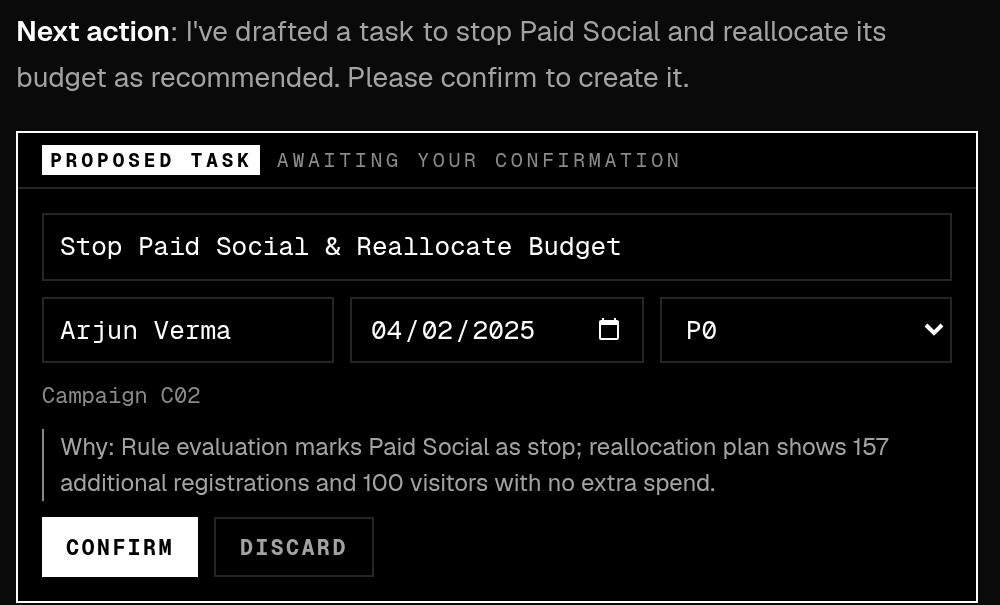
\includegraphics[width=7.3cm]{img/copilot-proposal.png}};
\node[anchor=north west,inner sep=0] at (15.85,-16.25) {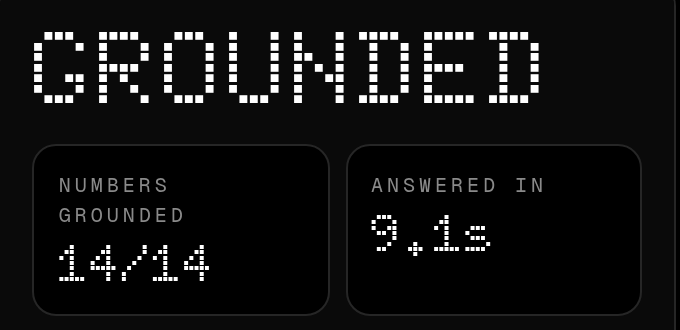
\includegraphics[width=3.45cm]{img/copilot-verdict.png}};
\blk{19.55}{16.3}{3.6}{\fs{7.6}{9}\color{fg2}The copilot's own verdict panel for this answer.}
\blk{23.5}{11.75}{9.07}{\fs{8.5}{10.6}\color{fg2}
  \textbf{\color{fg}Example, 31 Mar.} Asked ``what should we do?'', the copilot flags \textbf{Paid Social at ₹256} per registration: past its ₹150 bet line and the ₹110 portfolio line (14 days, 75 registrations). Creator Partners is at ₹134. It proposes moving \textbf{₹16,800} to four cheaper campaigns for \textbf{+157 registrations, +100 visitors}, then drafts this task. \textbf{Nothing changes until someone presses Confirm.}\\[4pt]
  \textbf{\color{fg}Grounding:} in this answer 14 of 14 numbers matched tool output; across the 30-question test, 89\% did (29/30 answers correct).\\[4pt]
  \textbf{\color{fg}Dashboard:} the Bets page shows each signal live, Overview ranks the next actions, and Decisions logs every call with its outcome.}

\footer{Signal lines are stored per bet in the app (Bets page); portfolio rule: scale ≤ 0.8×, stop ≥ 1.5× the 14-day portfolio CPR (₹73.58 on 31 Mar)\tg{A}. Readings: the app's engine replaying the RISA dataset\tg{D}. \gS{} scale · \gW{} watch / change · \gX{} stop.\quad \textbf{Rules, reallocation, copilot: README.pdf §5.7–5.8, §8.}}
\end{scope}
\end{tikzpicture}
\end{document}
